\documentclass[main.tex]{subfiles}

\begin{document}
\sloppy


\vspace{1.0cm}

\section{Introduzione}\label{sec:Intro}
Nel mondo dell'eventistica progettare anticipatamente su una piattaforma virtuale palchi e show, è una pratica sempre più diffusa e viene realizzata attraverso programmi detti \say{Previsualizer}. Solitamente vengono utilizzati software\cite{capture} ad-hoc, closed-source e molto costosi, con una resa qualitativa molto elevata. Esistono anche dei software gratuiti, molto spesso già inclusi nei sistemi di controllo luci, che però omettono molte funzionalità essenziali ed hanno una resa grafica nettamente inferiore.\newline

Lo scopo del progetto CPGDTF-Importer è quello di realizzare un previsualizer open-source basato su \say{Unreal Engine}\cite{UnrealEngine}, un importante ed affermato software ed engine grafico per la realizzazione di videogiochi, sviluppato dalla \say{Epic Games}. Unreal Engine (abbreviato con \say{UE}) è gratuito, open-source, ha un rendering visivo fotorealistico e mette a disposizione un sistema di plugin con i quali è possibile integrare l'importazione di file non nativi, automatizzare i processi di creazione di \say{oggetti} utilizzabili all'interno dell'engine, oppure definire il comportamento degli stessi. UE dispone di una libreria di plugin sviluppati internamente dalla Epic Games tra cui figura \say{DMXEngine}, che già implementa protocolli standard per la gestione di luci e palchi, e già detta delle basi per sviluppare un proprio plugin nel medesimo contesto.  
\newline
CPGDTF-Importer è una fork di DMXEngine ed è, in particolare, un plugin per l'\say{editor} di UE, ovvero quella sezione che permette la creazione di mondi che, nel nostro caso, consisterebbero in palcoscenici virtuali. Il plugin lavorerà principalmente su 3 livelli:
\begin{itemize}
    \item Importazione di luci da un formato standard (GDTF \cite{GDTF}, esposto nella sezione \ref{subsec:1_gdtf}), negli \say{Actor} di UE.
    \item Importazione di luci sotto forma di Attori all'interno di mondi e gestione delle loro impostazioni.
    \item Simulazione in real-time del comportamento delle fixture, il più possibile vicino alla realtà.
\end{itemize}

\subsection{Anatomia di una fixture}\label{subsec:1_fixtureAnatomy}
Le luci (che chiameremo anche \say{fari} o \say{fixture}) utilizzati nel mondo dell'eventistica sono dei macchinari di vario tipo e dimensioni che hanno il compito di generare luce di forme e colori differenti. Le fixture che ci interessano sono quelle utilizzate sia come illuminazione di oggetti, come ad esempio quelle frontali che illuminano un attore in teatro, che come effettistica, ovvero le luci che fanno gli effetti aerei ai concerti. Storicamente le luci nascono come semplici fari monocolore a cui si potevano applicare a mano dei filtri davanti la sorgente luminosa ed a cui si poteva solamente regolare l'intensità attraverso apparecchiature chiamate \say{dimmer}. Solo a partire dagli anni '90 sono entrate in commercio le prime fixture intelligenti, ovvero con la possibilità di essere controllate da remoto attraverso una console luci sfruttando il protocollo DMX \cite{DMX}. 

\subsubsection{Luci statiche e dinamiche}\label{subsec:1_1_fixtureTypes}
Le fixture possono essere classificabili come statiche o dinamiche. Le fixture dette \say{statiche} sono fixture che sono formate da un unico \say{blocco} (che GDTF chiama \say{geometrie}, mentre Unreal Engine chiama \say{SceneComponents}) e che, fisicamente, non si muovono. Sono quelle più semplici nonché il primo tipo di faro entrato in commercio.
\begin{figure}[H]
    \centering
    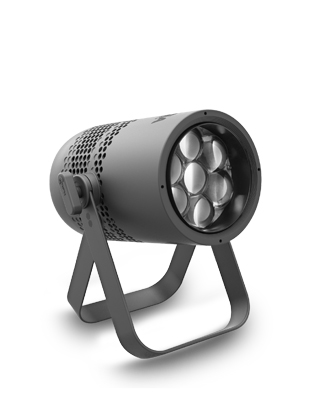
\includegraphics[width=0.36\linewidth]{img/introduzione/staticFixtureExample.jpg}
    \caption{Esempio di fixture statica. Immagine da \cite{fig_1_fixtureStatic}.}
    \label{fig:1_staticFixture}
\end{figure}
\noindent Le fixture dette invece \say{dinamiche} (chiamate anche \say{Teste mobili}) sono composte da più geometrie collegate tra loro da motori, in modo che quella responsabile di emettere il fascio di luce possa roteare, di solito su due assi. La geometria che viene poggiata per terra o appesa viene chiamata \say{base}, quella che emette luce \say{testa}.
\begin{figure}[H]
    \centering
    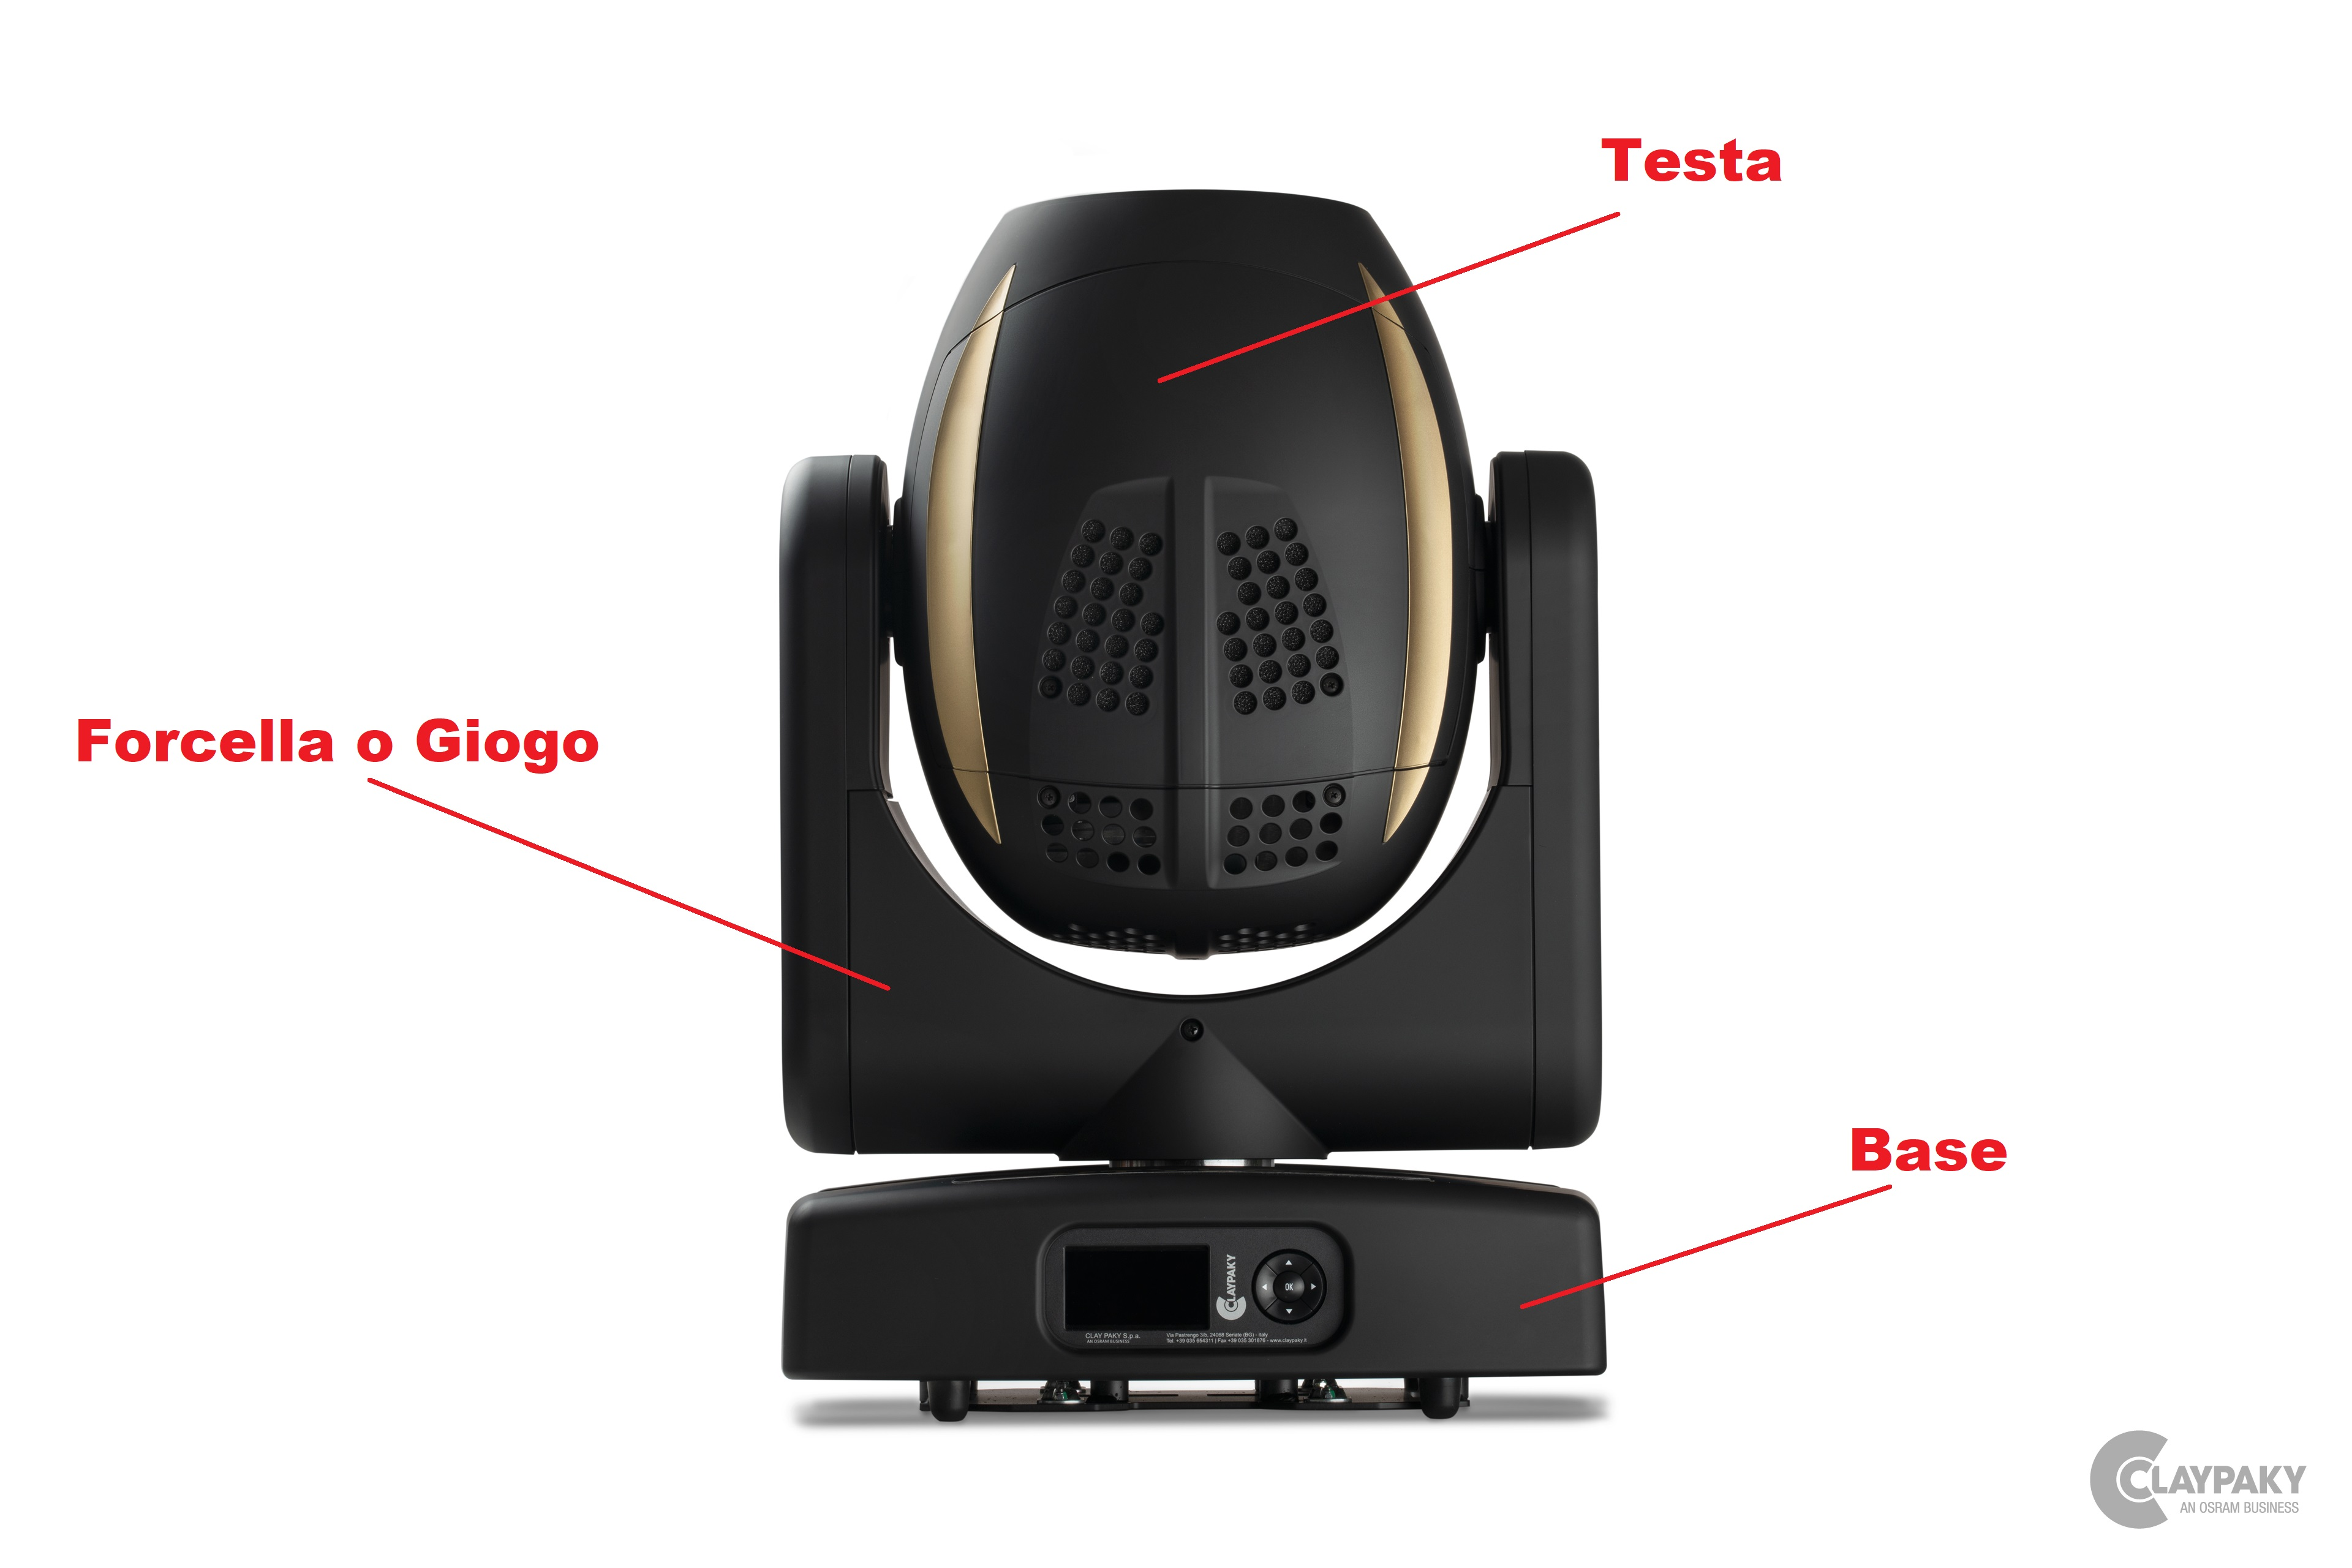
\includegraphics[width=0.65\linewidth]{img/introduzione/dynamicFixtureAnatomy.jpg}
    \caption{Geometrie di un faro dinamico. Immagine originale da \cite{fig_1_xtylos}.}
    \label{fig:1_DynamicFixture}
\end{figure}

\subsubsection{Moduli di una luce}\label{subsec:1_1_modules}
All'interno della testa, così come all'interno delle fixture statiche, è presente una sorgente luminosa che può essere bianca se il faro utilizza una sintesi colore sottrattiva, oppure colorata se il faro utilizza una sintesi colore additiva. La luce viene fatta passare attraverso vari moduli che ne alterano il colore, la messa a fuoco e la forma fino ad uscire dalla lente principale collocata ad una estremità della testa. Su praticamente tutti i fari in commercio non è possibile montare moduli custom o invertirli con quelli di un altro faro. \newline
I moduli che verranno toccati in questo progetto sono i seguenti:
\begin{itemize}
    \item \textbf{Ruote colori e gobo}: Sono delle ruote in cui sono presenti degli slot contenenti dei filtri colori o delle forme. Hanno sempre uno slot libero in cui la luce può passare senza essere modificata e, girando, possono mettere \say{in mezzo} alla luce uno slot alla volta.
    \item \textbf{Sintesi e correzione dei colori}: Nelle luci a sintesi additiva troviamo LED di colori differenti (RGB + Bianco, Ambra, Lime, UV, etc); nelle luci a sintesi sottrattiva invece abbiamo una luce bianca e delle flag CMY che vengono inserite davanti per regolarne il colore. Esistono anche dei filtri, sempre sottrattivi, per effettuare color correction.
    \item \textbf{Sagomatore}: È un sistema composto da quattro lame che possono essere inserite nel fascio di luce da direzioni differenti e possono essere inclinate, in modo da ritagliare in maniera precisa triangoli e quadrilateri per fare puntamenti.
    \item \textbf{Iris}: Sono delle lame circolari che entrano nel fascio di luce da tutte le direzioni e si occupano di ridurne la dimensione. Il funzionamento è analogo al diaframma di una fotocamera.
    \item \textbf{Frost}: È un filtro atto a rendere soffusa la luce, smorzando i bordi di eventuali figure che si stanno proiettando.
\end{itemize}
I moduli solitamente funzionano sottrattivamente: per ogni modulo a partire dalla fonte luminosa, andiamo ad occluderla mano a mano per disegnare la forma che vogliamo ottenere.
\begin{figure}[H]
    \centering
    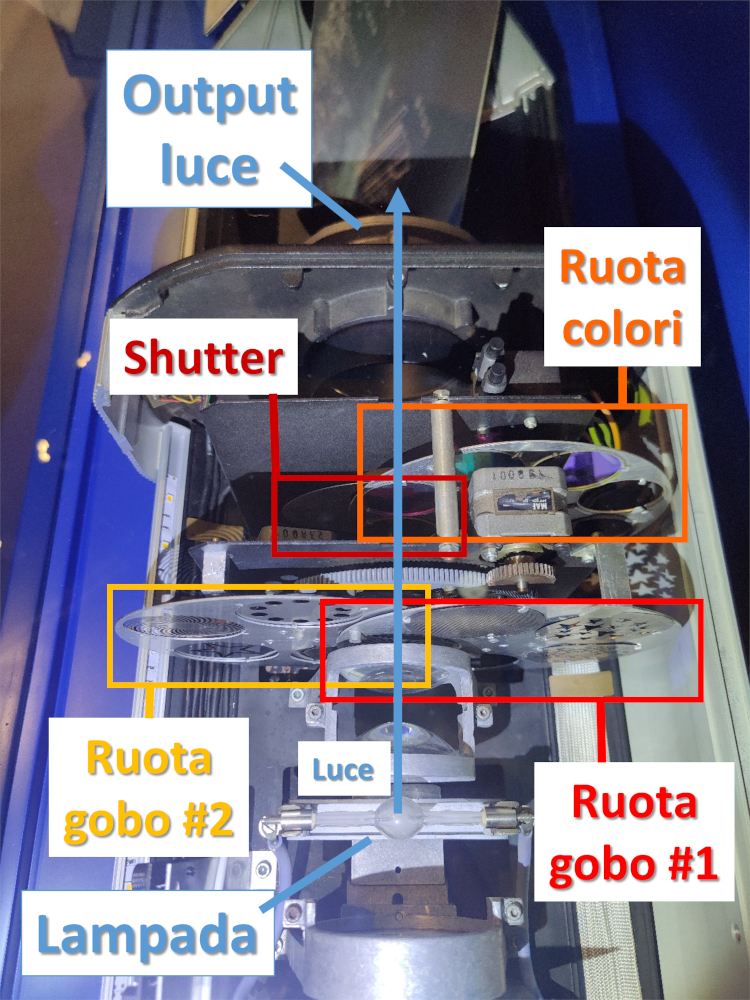
\includegraphics[width=0.8\linewidth]{img/introduzione/fixtureModules.jpg}
    \caption{Fotografia di una vecchia fixture aperta, in cui sono visibili in maniera chiara la sorgente luminosa ed i vari moduli che la compongono.}
    \label{fig:1_FixtureModules}
\end{figure}

%\clearpage
\subsubsection{Protocollo DMX}\label{subsec:1_1_dmx}
Oggi giorno, quasi tutte le fixture che vengono usate sono intelligenti e, come citato sopra, vengono controllate via DMX. DMX è un protocollo unidirezionale in cui un master, che solitamente è una console luci, invia 44 volte al secondo un array di 512 byte (chiamato \say{Universo DMX}) alle varie fixture che funzionano come slave. Le luci hanno memorizzato un offset all'interno di questo array chiamato \say{Indirizzo DMX} che viene impostato manualmente su ognuna dall'operaio che le monta su un palcoscenico. Ogni volta che arriva un nuovo pacchetto DMX la luce inizierà a leggere la sua sezione di dati a partire dall'indirizzo/offset specificato. Ogni byte che legge è chiamato \say{canale DMX} e, solitamente, corrisponde al valore da assegnare ad una diversa \say{funzionalità} (chiamata anche \say{feature}, o \say{attributo}) della luce.
\begin{figure}[H]
    \centering
    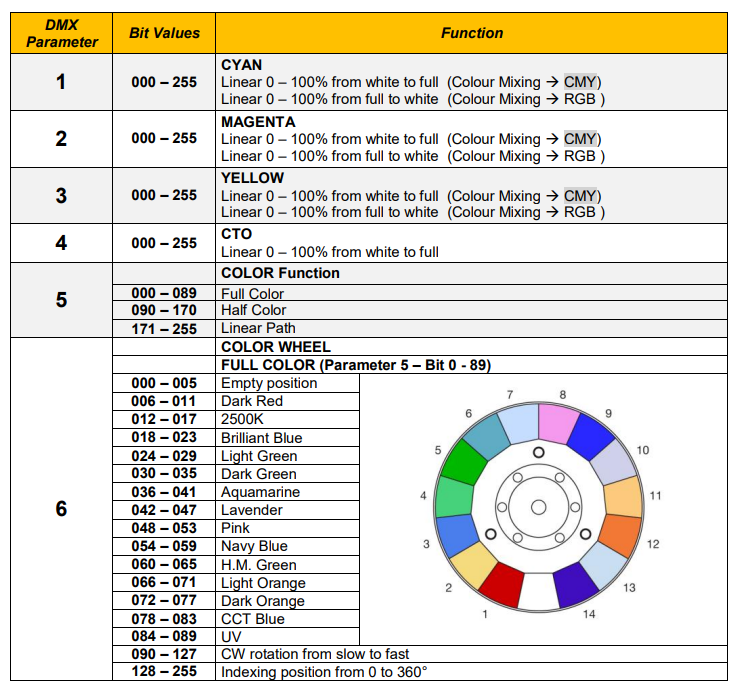
\includegraphics[width=0.65\linewidth]{img/introduzione/dmxChannelDescExample.png}
    \caption{Esempio di canali DMX presi da \cite{fig_1_dmxChart}. Se il canale 1 di questa luce viene portato a FULL (255), la luce si colorerà di azzurro. Se, invece, il canale 6 viene impostato al valore 50, si colorerà di rosa.}
    \label{fig:1_dmxChannelsExample}
\end{figure}

\noindent Alcune fixture possono supportare più modalità di controllo, che possono andare ad attivare o disattivare funzionalità della luce stessa, oppure possono permettere il controllo più preciso di alcuni attributi; introducendo quindi nuovi canali da controllare o riordinando quelli già esistenti. 


\subsection{GDTF}\label{subsec:1_gdtf}
GDTF - \textit{General Device Type Format} - è un formato per descrivere fixture nella maniera più accurata possibile. È stato sviluppato da MAlighting (azienda produttrice del sistema di controllo luci attualmente più usato in show medio-grandi), Robe (uno dei leader mondiali nello sviluppo e realizzazione di luci per l'eventistica) e Vectorworks (un software di CAD/Design anch'esso molto usato nella progettazione e previsualizzazione di palcoscenici). 
\newline

\noindent Un file GDTF è essenzialmente un pacchetto contenente all'interno i modelli 3D delle varie geometrie che compongono un faro, le texture delle sue gobo/animazioni/prismi/etc ed un file in formato XML contenente una descrizione esaustiva delle caratteristiche del faro. \newline
Dei vari dati contenuti in questo XML a noi ci interessano principalmente:
\begin{itemize}
    \item Informazioni e texture delle ruote colori e gobo.
    \item Informazioni sui valori di fade e accelerazione per l'interpolazione delle varie componenti fisiche.
    \item Modelli 3D, geometrie di un faro e come sono in relazione tra di loro.
    \item Informazioni sui vari canali DMX e sulle varie modalità DMX.
\end{itemize}

\subsubsection{Ruote}\label{subsec:1_2_wheels}
Nel nodo \lstinline{Wheels} all'interno del file XML viene definita una lista di ruote presenti all'interno del faro. Ogni ruota, rappresentata da un nodo \lstinline{Wheel}, può avere un nome e dentro ciascuna troviamo una lista di \lstinline{Slot} che rappresentano ognuno un elemento della ruota. Ogni slot ha anch'esso un nome e può avere degli attributi opzionali quali:
\begin{itemize}
    \item \lstinline{Color}: Il colore di uno slot presente su una color wheel.
    \item \lstinline{MediaFileName}: Nome del file PNG contenente la texture di questo slot, utilizzato per le ruote gobo ed animazione.
\end{itemize}
I prismi vengono comunque classificati come ruote, dove ogni slot rappresenta un tipo diverso di prisma. In questi casi avranno come figli dei nodi \lstinline{Facet} rappresentanti le facce di un prisma, in cui ne viene definito il colore, la rotazione, la traslazione e la grandezza della faccia.
\begin{figure}[H]
    \centering
    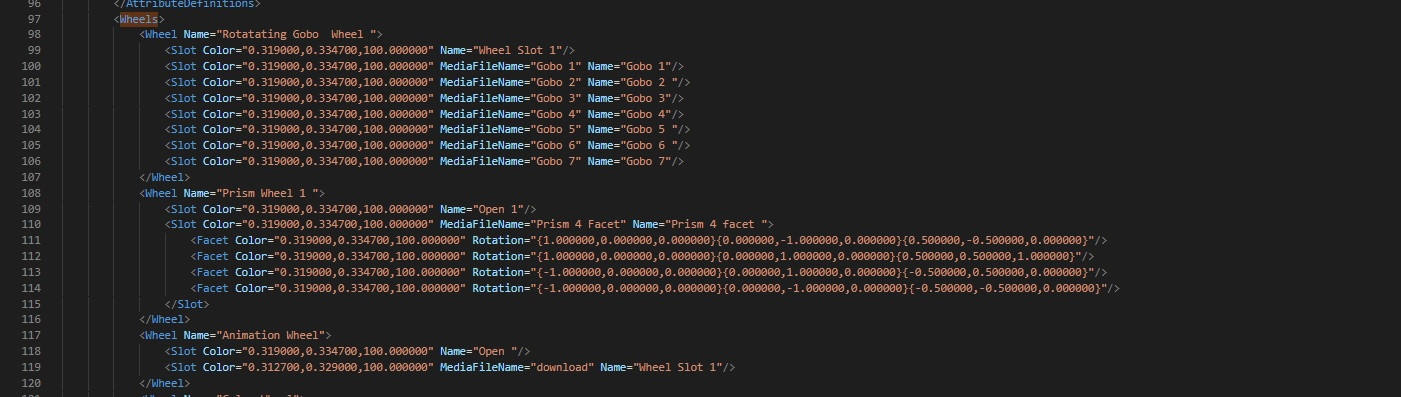
\includegraphics[width=1\linewidth]{img/introduzione/GDTFwheelExample.jpg}
    \caption{Nodo \lstinline{Wheels} in un file GDTF.}
    \label{fig:1_gdtfWheelExample}
\end{figure}

\subsubsection{Geometrie}\label{subsec:1_2_geometries}
Il nodo \lstinline{Models} viene utilizzato per definire una lista di modelli 3D da importare. Per ciascuno può essere assegnato un nome e delle dimensioni per effettuare dello scaling al modello stesso. 

I vari modelli che vengono importati vengono poi usati all'interno del nodo \lstinline{Geometries}, che va a definire una gerarchia di geometrie, specificando i punti di interconnessione tra le varie e gli assi e centri di rotazione di ciascuna. Alcune geometrie, come ad esempio \lstinline{Beam}, sono particolari, perché rappresentano un punto in cui la luce può essere emessa dalla fixture.\newline
Le varie funzionalità di una fixture sono implementate all'interno di una particolare geometria, o meglio, \textit{riguardano} una geometria.
\begin{figure}[H]
    \centering
    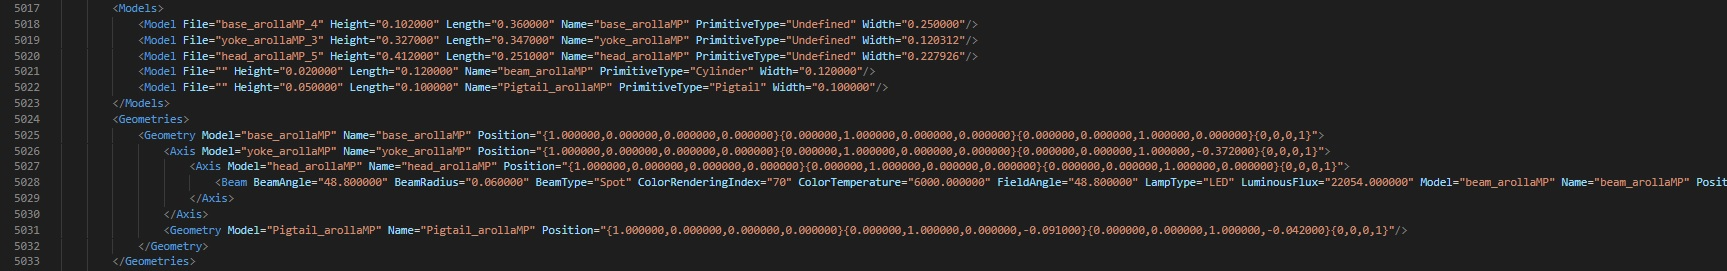
\includegraphics[width=1\linewidth]{img/introduzione/GDTFgeometriesExample.jpg}
    \caption{Esempio di nodi \lstinline{Models} e \lstinline{Geometries} in un file GDTF.}
    \label{fig:1_gdtfGeometriesExample}
\end{figure}

\subsubsection{Modalità e canali DMX}\label{subsec:1_2_dmxchannels}
Il nodo \lstinline{DMXMode} raccoglie tutte le modalità di funzionamento di un faro, che vengono enumerate dal nome. Dentro ciascuno di questi nodi troviamo la descrizione dettagliata dei canali DMX di una fixture, disposta in maniera gerarchica:
\begin{itemize}
    \item I primi figli di un DMXMode sono i nodi \lstinline{DMXChannel} che rappresentano un canale dmx \say{fisico}. Gli attributi principali di un DMXChannel sono: \begin{itemize}
            \item \lstinline{Offset}: Offset del canale fisico rispetto all'indirizzo di partenza di una fixture.
            \item \lstinline{Highlight}: Valore dmx applicato al canale quando la fixture viene messa in modalità \say{Highlight}, ovvero una modalità usata per evidenziare e trovare una determinato faro tra i tanti montati su un palcoscenico.
            \item \lstinline{Geometry}: Nome della geometria controllata da questo canale.
            \item \lstinline{InitialFunction}: Nome della \lstinline{ChannelFunction} da eseguire come valore default del canale, espresso nella forma: \lstinline{NomeGeometria_AttributoLogicalChannel.AttributoChannelFunction.NomeChannelFunction}
        \end{itemize}
    \item I figli di un DMXChannel sono i nodi \lstinline{LogicalChannel}. Su alcune fixture un canale dmx fisico può controllare funzionalità differenti, per questo motivo esiste una distinzione tra LogicalChannel e DMXChannel rappresentante il canale fisico. I LogicalChannel all'interno dello stesso DMXChannel sono mutualmente esclusivi. Gli attributi principali di un LogicalChannel sono: \begin{itemize}
            \item \lstinline{Snap}: Se lo snap è abilitato vuol dire che questo attributo non deve essere interpolato quando andiamo a fare la preview del faro, ma deve saltare direttamente a quel valore, poiché, fisicamente su una fixture vera, la feature non è controllata da un motore. Un esempio è il controllo della luminosità di un LED, che è istantaneo.
            \item \lstinline{Attribute}: Feature controllata da questo LogicalChannel.
        \end{itemize}
    \item Sotto i LogicalChannel abbiamo i \lstinline{ChannelFunction}, che rappresentano una funzionalità specifica dell'attributo indicato nel LogicalChannel padre. Ad esempio, l'attributo del padre potrebbe essere \lstinline{Shutter} e come figli potrebbe avere due ChannelFunction di tipo \lstinline{StrobeRandom} e \lstinline{LinearStrobe}: Entrambi i ChannelFunction fanno uso dello stesso attributo fisico, lo shutter, ma di fatto sono due funzionalità differenti. Gli attributi principali di una ChannelFunction sono: \begin{itemize}
            \item \lstinline{Name}: Nome della ChannelFunction.
            \item \lstinline{Attribute}: Feature specifica di questo ChannelFunction, che riguarda comunque la feature generale specificata nel nodo LogicalChannel padre.
            \item \lstinline{DMXFrom}: Valore DMX in cui questa ChannelFunction inizia nel DMXChannel. Non esiste un attributo DMXTo indicato esplicitamente in GDTF; viene calcolato utilizzando il valore DMXFrom della ChannelFunction successiva, oppure, se è l'ultima ChannelFunction nella lista, il valore massimo che può assumere il DMXChannel.
            \item \lstinline{Default}: Valore default quando questa ChannelFunction viene richiamata.
            \item \lstinline{PhysicalFrom}: Valore fisico di partenza che questo attributo può raggiungere in un faro vero. Esempio: se l'attributo è \lstinline{Zoom}, corrisponde all'apertura che il fascio di luce avrà quando il valore DMX è uguale a DMXFrom.
            \item \lstinline{PhysicalTo}: Valore fisico di arrivo che questo attributo può raggiungere in un faro vero. Esempio: se l'attributo è \lstinline{Zoom}, corrisponde all'apertura che il fascio di luce avrà quando il valore DMX è uguale a DMXTo.
            \item \lstinline{RealFade}: Tempo in secondi che questa feature impiega su un faro vero per passare da PhysicalFrom a PhysicalTo, usato per l'interpolazione.
            \item \lstinline{RealAcceleration}: Tempo in secondi che questa feature impiega su un faro vero per passare dall'essere ferma a raggiungere la velocità di movimento massima, usato per l'interpolazione.
            \item \lstinline{Wheel}: Opzionale, nome della ruota a cui questo attributo fa riferimento.
        \end{itemize}
    \item Infine abbiamo i \lstinline{ChannelSet} che rappresentano delle macro o valori precisi che una ChannelFunction può assumere. Gli attributi di un ChannelSet sono: \begin{itemize}
            \item \lstinline{Name}: Nome/DisplayName del channel set.
            \item \lstinline{DMXFrom}: Valore DMX in cui questo ChannelSet inizia nel DMXChannel. Analogamente alle ChannelFunction, non esiste un attributo DMXTo, che verrà calcolato allo stesso modo loro, eccezion fatta che come valore massimo non si userà quello del DMXChannel, bensì quello della ChannelFunction. 
            \item \lstinline{PhysicalFrom}: Funzionamento analogo alle ChannelFunction. Se non viene specificato, può essere calcolato come proporzione:
            \[PysicalFrom_{CS} : PhysicalRange_{CF} = DMXFrom_{CS} : DMXRange_{CS}\]
            Dove $PhysicalRange$ e $DMXRange$ si ottengono calcolando il rispettivo valore To meno il rispettivo valore From.
            \item \lstinline{PhysicalTo}: Funzionamento analogo alle ChannelFunction. Se non viene specificato, può essere calcolato come proporzione:
            \[PysicalTo_{CS} : PhysicalRange_{CF} = DMXTo_{CS} : DMXRange_{CS}\]
            Dove $PhysicalRange$ e $DMXRange$ si ottengono calcolando il rispettivo valore To meno il rispettivo valore From.
            \item \lstinline{WheelSlotIndex}: Se la ChannelFunction padre è collegata ad una ruota, è l'identificativo dello slot nella ruota che dovrà essere attivo quando il valore del canale DMX fisico si trova nel range di questo ChannelSet.
        \end{itemize}
\end{itemize}
\begin{figure}[H]
    \centering
    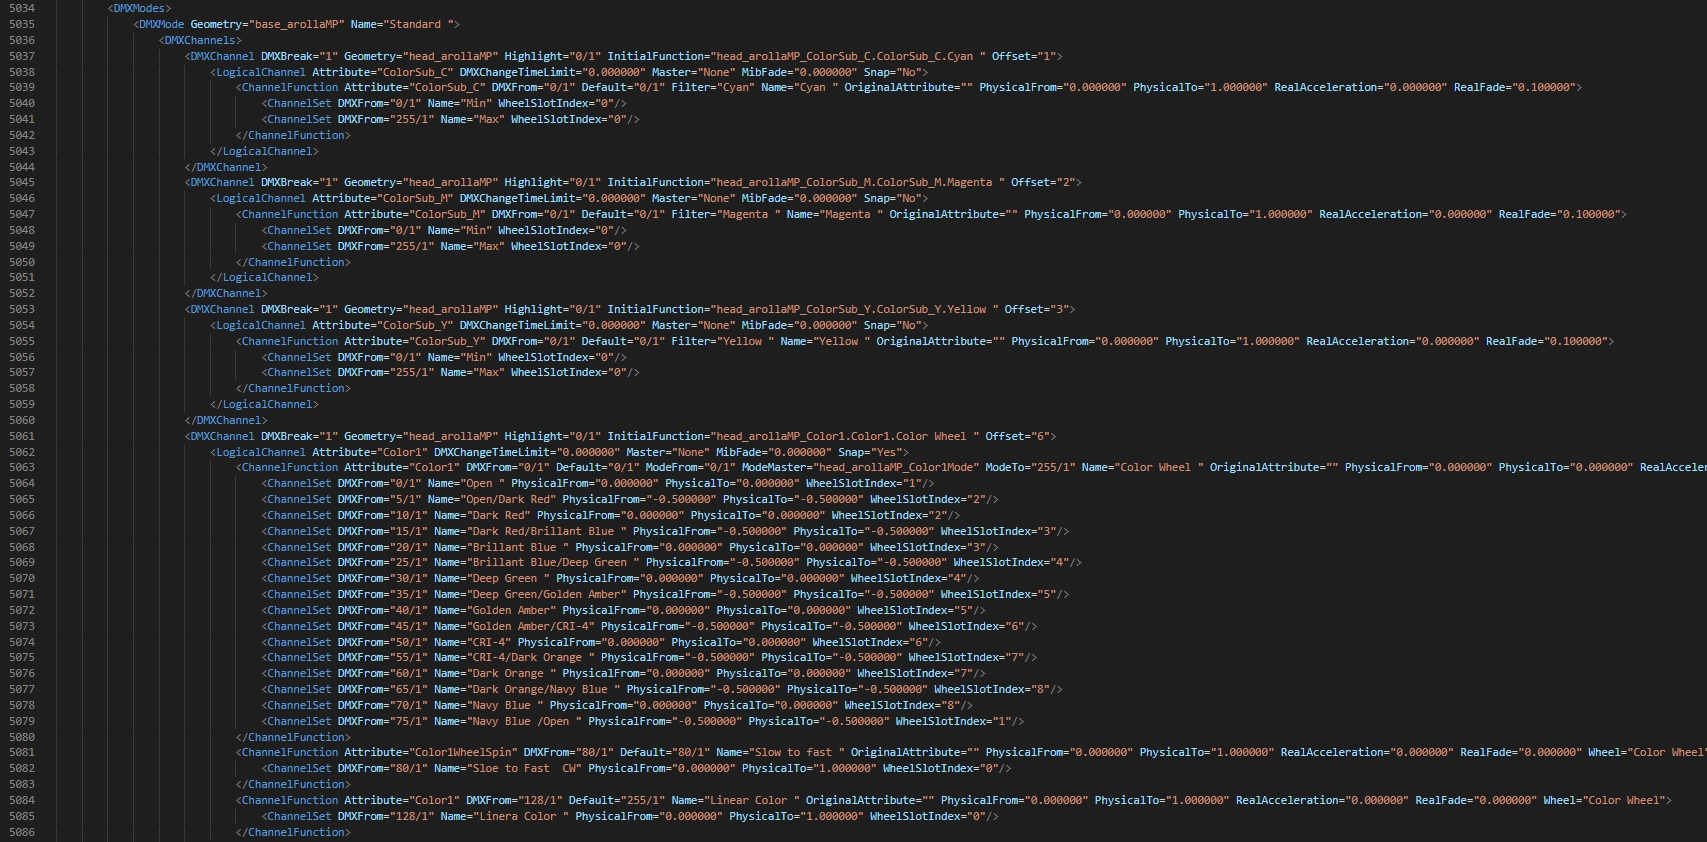
\includegraphics[width=1\linewidth]{img/introduzione/GDTFdmxExample.jpg}
    \caption{Esempio di nodi rappresentanti la descrizione di un canale DMX in un file GDTF.}
    \label{fig:1_gdtfDmxExample}
\end{figure}

%\clearpage
\subsection{Terminologia di Unreal Engine}\label{subsec:1_dataStructsUE}
Qui sotto elencate tutti tutti i termini che si riferiscono a concetti e oggetti di Unreal Engine.
\begin{itemize}
    \item \textbf{Actor}: Un attore è un qualsiasi oggetto su Unreal Engine che può essere piazzato in un mondo. Può contenere una gerarchia di Componenti che lo caratterizzano.
    \item \textbf{Component}: I componenti sono un tipo di oggetto che un attore può possedere.
    \item \textbf{Material}: Un materiale è un asset che può essere applicato ad un componente e ne va a definire il suo comportamento. Un materiale viene programmato tramite un grafo che ha, come output, una texture.
    \item \textbf{MaterialInstance}: Istanza di un materiale con un valore impostato staticamente per ogni suo parametro. Utilizzato per avere più oggetti simili, ma con qualche differenza tra loro che non richiede la creazione completa di un nuovo materiale.
    \item \textbf{MaterialFunction}: Materiali che si comportano come una funzione in un normale linguaggio di programmazione: prendono degli input, hanno degli output e possono essere richiamate più volte in grafi differenti.
    \item \textbf{MaterialExpression}: Nodi di un grafo di un Material.
    \item \textbf{MaterialExpressionParameter}: Tipo di MaterialExpression che permettono di controllare i parametri del materiale esternamente.
    \item \textbf{MaterialExpressionFunctionCall}: Tipo di MaterialExpression che implementa una chiamata ad una MaterialFunction.
    \item \textbf{MaterialExpressionCustom} o \say{CustomExpression}: Tipo di MaterialExpression che prende degli input e ritorna degli output. Mentre una MaterialExpressionFunctionCall elabora gli output utilizzando il grafo di una MaterialFunction, una MaterialExpressionCustom esegue codice vero e proprio scritto in HLSL, un linguaggio C-like utilizzato per la scrittura di Shader.
\end{itemize}


\subsection{Informazioni sul tirocinio}\label{subsec:1_tirocinio}
CPGDTF-Importer è un progetto sviluppato dalla \say{Clay Paky}, azienda italiana leader mondiale nella progettazione e realizzazione di luci per concerti, architettura e teatri, per cui ho svolto il tirocinio curricolare. Lo sviluppo ha avuto inizio nel Maggio 2022 da un altro tirocinante che ha fatto un fork del plugin originale sviluppato dalla Epic Games ed ha iniziato ad aggiungere funzioni che, nonostante fossero basilari, mancavano totalmente. Il plugin originale leggeva solamente quali fossero i componenti di una fixture, i suoi canali e poche altre informazioni. Utilizzava sempre modelli 3D e ruote gobo predefinite, non importava i valori di fade e accelerazione per l'interpolazione, mancavano moltissime features delle fixture, quelle esistenti funzionavano male, e molto altro ancora. Il tirocinante precedente, dopo aver speso quasi tutto il periodo del suo tirocinio a fare ricerca su come funzionasse il plugin originale, ha gettato delle basi per iniziare ad estenderlo e per completare l'importazione di tutti i dati e file da un GDTF. Ha infine scritto delle documentazioni abbastanza esaustive dell'intero plugin.\newline

Al mio arrivo in ClayPaky mi è stato affidato il progetto con l'obiettivo di implementare nuove funzionalità delle fixtures in modo da poter arrivare a simulare completamente tutti i fari dell'azienda.

Dopo aver speso un primo periodo a prendere conoscenza con la codebase mi sono reso conto di quanto buona parte del codice necessitasse di un refactoring. In particolare ho riscontrato difficoltà nell'implementare nuove features, sia perché il codice che si occupava del rendering dell'illuminazione non fosse in alcun modo modulare e sia perché la gerarchia di classi che le gestisce fosse mal disegnata e con tanto codice duplicato. 

Solamente dopo aver risolto questi grossi problemi strutturali nel codice e dopo aver fatto funzionare correttamente l'interpolazione ho potuto dedicarmi all'implementazione effettiva di nuove features. 

%\clearpage %TODO CHECK IF THIS IS STILL NEEDED
\subsection{Struttura della tesi}\label{subsec:1_thesisInfo}
L'elaborato è articolato come segue. Ogni capitolo rappresenta una milestone del progetto:
\begin{itemize}
    \item \textbf{Capitolo \ref{sec:Intro}, Introduzione}. %We like recurion
    \item \textbf{Capitolo \ref{sec:RenderingPipeline}, Design di una pipeline di rendering}: In questo capitolo verrà analizzata l'implementazione originale con la quale veniva effettuato il rendering dell'illuminazione di ogni singola fixture. Verranno evidenziati i problemi e mostrate idee per risolverli. Infine verrà anche esposta l'implementazione per la generazione di una pipeline vera e propria per il rendering dei vari moduli di una luce. 
    \item \textbf{Capitolo \ref{sec:FixtureComponentHierachy}, Redesign gerarchia dei FixtureComponent}: Tratta l'analisi della vecchia gerarchia dei FixtureComponent, ovvero quelle classi responsabili di controllare ogni singola feature che compone una fixture. Vengono proposte nuove idee di implementazione e mostrati quali dati e metodi servirebbe mettere a disposizione alle classi che implementano la singola feature.
    \item \textbf{Capitolo \ref{sec:Interpolation}, Nuovo approccio all'interpolazione}: All'interno di questo capitolo vengono velocemente esposti i problemi dell'attuale classe che controlla l'interpolazione, ovvero il controllo del movimento dei motori virtuali. Successivamente viene mostrata la nuova implementazione della classe, spiegando i vari problemi che si sono verificati durante la scrittura del codice e come sono stati risolti.
    \item \textbf{Capitolo \ref{sec:NewFeatures}, Implementazione di nuove funzionalità alle fixtures}: Una volta sistemata la struttura del plugin e reso comodo e meno error-prone l'implementazione di nuove feature, viene descritta come sono state pensate e implementate le due funzionalità che sono state aggiunte a CPGDTF-Importer.
    \item \textbf{Capitolo \ref{sec:End}, Conclusioni}: In questo capitolo conclusivo vengono sintetizzati i problemi generali emersi durante lo sviluppo con GDTF ed Unreal Engine. Inoltre, vengono valutati futuri sviluppi con l'azienda che ha acquisito ClayPaky lo scorso Marzo (Arri), durante il mio periodo di tirocinio, e con Epic Games stessa.
\end{itemize}


\end{document}